\documentclass[leqno]{beamer}

\usepackage{default}
\usepackage[english]{babel}
\usepackage{amsmath,amsthm,amsfonts}
\usepackage[T1]{fontenc}
\usepackage[utf8]{inputenc}
\usepackage{lmodern}
\usepackage{enumerate}
\usepackage[noend]{algpseudocode}
\usepackage{fp}
\usepackage{calc}
\usepackage{tikz}
\usepackage{catchfile}

\usetikzlibrary{arrows,calc,decorations.pathmorphing,decorations.pathreplacing,shapes,fit}

\newcommand{\unitsize}{0.25cm}

\setlength{\rightskip}{0pt} % I want justifed text
\sloppy

\tikzset{%
  >=stealth',
  dotbase/.style={draw,thin,circle,minimum size=1*\unitsize,node distance=2*\unitsize,inner sep=0pt},
  dot/.style={dotbase,fill=black!80,font=\sffamily},
  dotpoint/.style={dot,minimum size=3pt},
  dotcross/.style={dotbase,fill=black!30},
}

\newcommand\dotcross[2]{%
  \node[dotcross] at (2*\unitsize * #1 - \unitsize, 2*\unitsize * #2 - \unitsize) {};
}

\newcommand<>\dotnode[4][]{%
  \node#5[#1] (#2) at (2*\unitsize * #3 - \unitsize, 2*\unitsize * #4 - \unitsize) {};
}

\newcommand\dotpoint[3][]{%
  \node[dotpoint,#1] at (2*\unitsize * #2 - \unitsize, 2*\unitsize * #3 - \unitsize) {};
}

\newcommand<>\dotmove[4][]{%
  \node#5[dot,#1] at (2*\unitsize * #2 - \unitsize, 2*\unitsize * #3 - \unitsize) {\scalebox{0.5}{\color{white}{#4}}};
}

\newcommand<>\dotdir[4][]{%
  \node#5[dot,#1] (X) at (2*\unitsize * #2 - \unitsize, 2*\unitsize * #3 - \unitsize) {};
  \draw[white,thick] (X) +(#4 * 45 : 0.375 * \unitsize) -- +(180 + #4 * 45 : 0.375 * \unitsize);
}

\newcommand<>\drawmove[5][]{%
  \draw#6[thick,#1]
    (2*\unitsize * #2 - \unitsize, 2*\unitsize * #3 - \unitsize)
    -- +(8 * #4 * \unitsize, 8 * #5 * \unitsize);
}

\newcommand\drawgrid[4]{%
  \draw[step=2*\unitsize,gray!30,very thin,shift={(-\unitsize, -\unitsize)}]
  (2*\unitsize * #1 - \unitsize, 2*\unitsize * #2 - \unitsize) grid (2*\unitsize * #3 + \unitsize, 2*\unitsize * #4 + \unitsize);
}

\newcommand\drawcross[2]{%
  \def\px{#1}
  \def\py{#2}
  \def\dx{-1}
  \def\dy{0}
  \def\rotleft{%
    \FPeval{tmpx}{neg(dy)}
    \FPeval{dy}{dx}
    \FPeval{dx}{tmpx}
  }
  \def\rotright{%
    \FPeval{tmpx}{dy}
    \FPeval{dy}{neg(dx)}
    \FPeval{dx}{tmpx}
  }
  \def\singlestep{%
      \FPeval{px}{px + dx}
      \FPeval{py}{py + dy}
      \dotcross{\px}{\py}
  }
  \def\crossside{%
    \singlestep
    \singlestep
    \singlestep
  }
  \def\crossarm{%
    \crossside
    \rotright
    \crossside
    \rotright
    \crossside
    \rotleft
  }
  \crossarm
  \crossarm
  \crossarm
  \crossarm
}

\newcommand<>{\onode}[1]{%
\begin{tikzpicture}[remember picture,overlay]#2
  \node (#1) at (0,0) {};
\end{tikzpicture}}

\DeclareMathOperator{\mv}{move}
\DeclareMathOperator{\dt}{dot}
\DeclareMathOperator{\ord}{ord}
\renewcommand{\L}[1]{{\sffamily L\textsubscript{#1}}}

\newcommand{\Zset}{\mathbb{Z}}
\newcommand{\Bbox}{\mathcal{B}}
\newcommand{\Cross}{\mathtt{Cross}}

\newcommand{\var}[1]{\textsl{#1}}
\algnewcommand\algorithmicforeach{\textbf{for each}}
\algdef{S}[FOR]{ForEach}[1]{\algorithmicforeach\ #1\ \algorithmicdo}%

\newcommand{\backupbegin}{
   \newcounter{finalframe}
   \setcounter{finalframe}{\value{framenumber}}
}
\newcommand{\backupend}{
   \setcounter{framenumber}{\value{finalframe}}
}

\mode<presentation>
{
  %\usetheme{Warsaw}
  \usetheme{Madrid}
  \usecolortheme{seahorse}
  \usefonttheme{professionalfonts}
  \setbeamercovered{transparent}
}

%\includeonlyframes{current}


\title[Morpion Solitaire 5D]{An upper bound of 84 for Morpion Solitaire 5D}

\author[Michalewski Nagórko Pawlewicz]{Henryk Michalewski, Andrzej Nagórko, \underline{Jakub Pawlewicz}}

\institute[Warsaw]
{
University of Warsaw
}

\date[5th August 2016]{28th Canadian Conference
on Computational Geometry\\\vspace{3mm} CCCG 2016}

\begin{document}

\AtBeginSection[]
{
  \begin{frame}<beamer>
    \frametitle{Outline}
    \tableofcontents[currentsection]
  \end{frame}
}

\begin{frame}
  \titlepage
\end{frame}

\begin{frame}
  \frametitle{Outline}
  \tableofcontents
  % You might wish to add the option [pausesections]
\end{frame}

\section{Morpion Solitaire}

\begin{frame}
\frametitle{Morpion Solitaire}

\begin{itemize}
\item A single-player paper-and-pencil game

{\footnotesize The goal is to find longest possible sequence of valid moves.}

\item Popularized in France in 70's by {\em Science \& Vie} magazine

{\footnotesize The magazine published long sequences found by its readers.}

\item Two interesting variants: 5T and 5D

\item Difficult for computers

\vspace{3mm}

{5T: \footnotesize The human record was obtained by C.-H. Bruneau in $1976$.

It was beat by NRPA (Monte Carlo) algorithm by Ch. Rosin in $2010$.

Rosin got best paper award at IJCAI 2011 for this work.
}

\vspace{3mm}

{5D: \footnotesize The human record was obtained by A.~Langerman in $1999$.

Beaten by H.~Hyyrö and T.~Poranen in 2006.

Rosin set the world record in 2011.
}
\end{itemize}

\end{frame}

\begin{frame}
\frametitle{Rules of Morpion Solitaire}
\begin{center}
  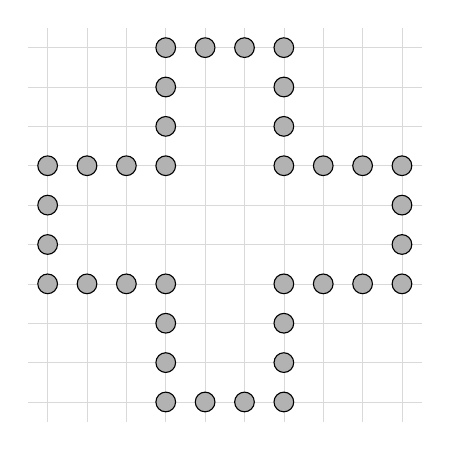
\begin{tikzpicture}
    \drawgrid{-3}{-3}{6}{6}
    \drawmove<2->{-3}{-1}{0}{1}
    \drawmove<3->{1}{-3}{-1}{1}
    \drawmove<4->{-3}{0}{1}{0}
    \drawmove<5>[red]{-2}{0}{1}{0}
    \drawmove<6>[red]{1}{0}{1}{0}
    \drawmove<7>{2}{0}{1}{0}
    \drawcross{0}{0}
    \dotmove<2->{-3}{-1}{1}
    \dotmove<3->{-1}{-1}{2}
    \dotmove<4->{1}{0}{3}
    \dotmove<5-6>[fill=red]{2}{0}{4}
    \dotmove<7>{2}{0}{4}
  \end{tikzpicture}

  \vspace{5mm}

  \begin{overlayarea}{\textwidth}{1cm}
    \begin{center}
      \only<1>{Initial position: $36$ dots arranged in a cross on a square grid.}
      \only<2>{A move: place a dot and draw a line (diagonal, horizontal or vertical) passing through the placed dot and four others.}
      \only<3>{Two lines may cross.}
      \only<4>{Vertical, diagonal and horizontal moves allowed.}
      \only<5>{Two parallel moves may not overlap,}
      \only<6>{neither touch (however allowed in 5T variant),}
      \only<7>{but allowed if disjoint.}
    \end{center}
  \end{overlayarea}

\end{center}
\end{frame}

\begin{frame}
\frametitle{The goal: find the longest sequence of moves}

\begin{columns}
\column{.25\textwidth}
  \begin{center}
    82 moves\\
    Rosin 2011
  \end{center}
\column{.75\textwidth}
  \begin{center}
  \begin{tikzpicture}
    \CatchFileDef\rosindmoves{data/82.moves}{}
    \drawgrid{-5}{-4}{9}{10}
    \foreach \x/\y/\dx/\dy in \rosindmoves {
      \drawmove{\x}{\y}{\dx}{\dy}
    }
    \drawcross{0}{0}
    \CatchFileDef\rosinddots{data/82.dots}{}
    \foreach \i/\d/\x/\y in \rosinddots {
      \dotmove{\x}{\y}{\i}
    }
  \end{tikzpicture}
  \end{center}
\end{columns}

\end{frame}

\begin{frame}
\frametitle{Upper bound}

The potential method gives a bound of 144 moves by Demaine et al. (2006).

A geometric analysis improves the upper bound to 121 moves by Kawamura et al. (2013).

\vspace{6mm}
{\bf We prove an upper bound of $84$.}

\vspace{6mm}
The proof has two main ingredients:

\vspace{3mm}
\begin{itemize}
  \item modelling the game by linear programming,
  \item limiting the size of the board by resizing process.
\end{itemize}

\end{frame}

\section{Linear Programming}

\begin{frame}
\frametitle{Morpion 5D position and marked graph}
\CatchFileDef\smallmoves{data/small.moves}{}
\CatchFileDef\smalldots{data/small.dots}{}
\begin{columns}
\column{.5\textwidth}
  \begin{center}
    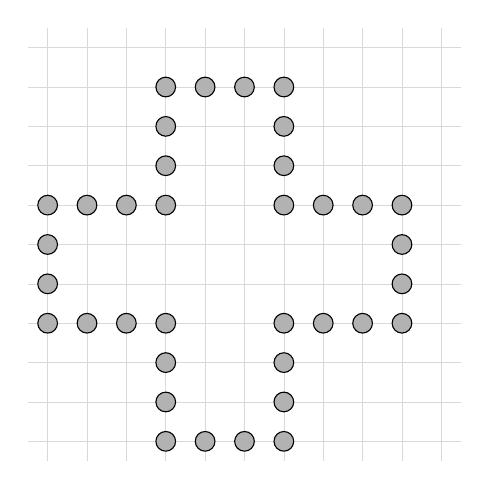
\begin{tikzpicture}
      \drawgrid{-3}{-3}{7}{7}
      \foreach \x/\y/\dx/\dy in \smallmoves {
        \drawmove{\x}{\y}{\dx}{\dy}
      }
      \drawcross{0}{0}
      \foreach \i/\d/\x/\y in \smalldots {
        \dotmove{\x}{\y}{\i}
      }
    \end{tikzpicture}
    Morpion 5D position
  \end{center}
\column{.5\textwidth}
  \begin{center}
    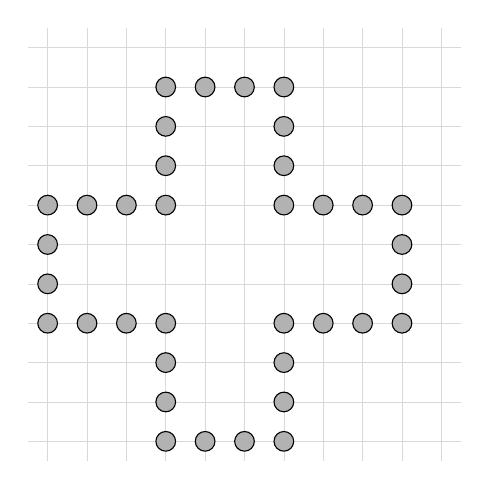
\begin{tikzpicture}
      \drawgrid{-3}{-3}{7}{7}
      \foreach \x/\y/\dx/\dy in \smallmoves {
        \drawmove{\x}{\y}{\dx}{\dy}
      }
      \drawcross{0}{0}
      \foreach \i/\d/\x/\y in \smalldots {
        \dotdir{\x}{\y}{\d}
      }
    \end{tikzpicture}   
    Marked Morpion 5D graph
  \end{center}
\end{columns}
\vspace{5mm}
Every Morpion 5D position has corresponding marked Morpion 5D graph.
\end{frame}

\begin{frame}
\frametitle{The board}
\begin{center}
  \begin{tikzpicture}
    \drawgrid{-6}{-4}{10}{8}
    \dotnode{A}{-6}{-4}
    \dotnode{C}{10}{8}
    \draw[dashed,blue] (A) rectangle (C);
    \only<1>{%
      \foreach \x in {-6, ..., 10}
        \foreach \y in {-4, ..., 8}
          \dotpoint{\x}{\y};
    }
    \only<2>{\drawcross{0}{0}}
  \end{tikzpicture}
\end{center}

\vspace{1mm}

\begin{overlayarea}{\textwidth}{1cm}
  \begin{center}
    \only<1>{We limit the board to rectangular grid $\Bbox\subset\Zset^2$ of points\\
    where the game is played.}
    \only<2>{$\Cross\subset\Bbox$ denote dots from the initial cross.}
  \end{center}
\end{overlayarea}

\end{frame}

\begin{frame}
\frametitle{Variables}
\begin{enumerate}
  \item $\dt_v$, $v\in\Bbox$.
  \begin{columns}
    \column{.5\textwidth}
      \centering
      \begin{tikzpicture}
        \drawgrid{0}{0}{4}{1}
        \dotnode[dotpoint]{v}{2}{0}
        \node[above left] at (v) {$v$};
        \node[below=2mm] at (v) {$\dt_v=0$};
      \end{tikzpicture}
    \column{.5\textwidth}
      \centering
      \begin{tikzpicture}
        \drawgrid{0}{0}{4}{1}
        \dotnode[dot]{v}{2}{0}
        \node[above left] at (v) {$v$};
        \node[below=2mm] at (v) {$\dt_v=1$};
      \end{tikzpicture}
  \end{columns}
  Desired property: $\dt_v=1$ iff dot was put at point $v$.
  \pause
  \item $\mv_{m, v}$, $m$ is a move, $v$ is a played dot (or marking of $m$).\\
  \emph{Move} $m$ is represented by five consecutive points on a horizontal, vertical or diagonal line: $m=\{d_1,d_2,d_3,d_4,d_5\}$, $v\in m$.\\
  \pause
  \begin{columns}
    \column{.25\textwidth}
      \centering
      \begin{tikzpicture}
        \drawgrid{1}{0}{5}{1}
        \foreach \x in {1, ..., 5} {
          \dotnode[dotpoint]{d\x}{\x}{0}
          \node[above] at (d\x) {$d_\x$};
        }
        \node[below=2mm] at (d3) {$\mv_{m,v}=0\vphantom{\begin{cases}0\\0\end{cases}}$};
      \end{tikzpicture}
    \column{.35\textwidth}
      \centering
      \begin{tikzpicture}
        \drawgrid{-1}{0}{5}{1}
        \drawmove{-1}{0}{1}{0}
        \dotmove{-1}{0}{}
        \dotmove{0}{0}{}
        \foreach \x in {1, ..., 3} {
          \dotnode[dot]{d\x}{\x}{0}
          \node[above] at (d\x) {$d_\x$};
        }
        \foreach \x in {4, 5} {
          \dotnode[dotpoint]{d\x}{\x}{0}
          \node[above] at (d\x) {$d_\x$};
        }
        \node[below=2mm] at (d2) {$\mv_{m,v}=0\vphantom{\begin{cases}0\\0\end{cases}}$};
      \end{tikzpicture}
    \column{.4\textwidth}
      \centering
      \begin{tikzpicture}
        \drawgrid{1}{0}{5}{1}
        \drawmove{1}{0}{1}{0}
        \foreach \x in {1, ..., 5} {
          \ifnum \x = 4
            \dotnode{d\x}{\x}{0}
            \dotdir{\x}{0}{0}
          \else
            \dotnode[dot]{d\x}{\x}{0}
          \fi
          \node[above] at (d\x) {$d_\x$};
        }
        \node[below=2mm] at (d3) {$
          \mv_{m,v}=
          \begin{cases}
            1&\text{if }v=d_4\\
            0&\text{if }v\neq d_4
          \end{cases}
        $};
      \end{tikzpicture}
  \end{columns}
  Desired property: $\mv_{m, v}=1$ iff a move was played by putting dot at $v$ and
  drawing line through points from set $m$.
\end{enumerate}

\end{frame}

\begin{frame}
\frametitle{Constraints: initial cross}
\begin{columns}
  \column{.55\textwidth}
    Let $v\in\Cross$\\
    Dots of cross must be put:

    \begin{block}{}
    \vspace{-18pt}
    \begin{equation}\label{eq:L1}
      \dt_v=1\tag*{\L1}
    \end{equation}
    \end{block}

    $v$ cannot be put by a move:

    \begin{block}{}
    \vspace{-15pt}
    \begin{equation}\label{eq:L2}
      \mv_{m,v}=0\quad\text{for all $m$ s.t. }v\in m\tag*{\L2}
    \end{equation}
    \end{block}
  \column{.03\textwidth}
  \column{.42\textwidth}
    \centering
    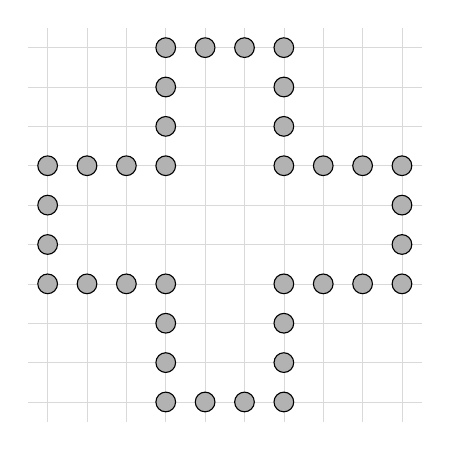
\begin{tikzpicture}
      \drawgrid{-3}{-3}{6}{6}
      \drawcross{0}{0}
    \end{tikzpicture}
\end{columns}
\end{frame}

\begin{frame}
\frametitle{Constraints: put dot}
Let $v\in\Bbox\setminus\Cross$.\\
If dot $v$ is put, there must be exactly one move by which it was put:
\begin{block}{}
\vspace{-9pt}
\begin{equation}\label{eq:L3}
  \dt_v=\sum_{m\text{ s.t. }v\in m} \mv_{m,v}\tag*{\L3}
\end{equation}
\end{block}
\begin{center}
  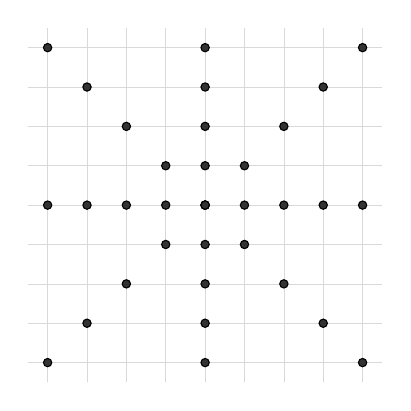
\begin{tikzpicture}
    \drawgrid{-4}{-4}{4}{4}
    \drawmove{-3}{3}{1}{-1}
    \foreach \i in {-4, ..., 4} {
      \dotpoint{\i}{0}
      \dotpoint{0}{\i}
      \dotpoint{\i}{\i}
      \dotpoint{\i}{-\i}
    }
    \dotdir{0}{0}{3}
  \end{tikzpicture}
\end{center}
\end{frame}

\begin{frame}
\frametitle{Constraints: conflicting moves, move needs dots}
Let $v\in\Bbox$ let $d$ be a direction
(vertical, horizontal or one of diagonals).\\
No move in the same direction should share a dot $v$:
\begin{block}{}
\begin{equation}\label{eq:L4}
  \dt_v\ge\sum_{\substack{m\text{ s.t. }v\in m\\m\text{ has direction }d}}\mv_m
  \quad\text{where }\mv_m=\sum_{w\in m}\mv_{m,w}\tag*{\L4}
\end{equation}
\end{block}
$\mv_m$ says whether a move through dots $m$ was played.
\begin{center}
  \begin{tikzpicture}
    \drawgrid{0}{0}{8}{0}
    \drawmove{1}{0}{1}{0}
    \foreach \x in {0, ..., 8}
      \dotnode[dotpoint]{d\x}{\x}{0};
    \draw[decorate,decoration={brace,amplitude=6pt,mirror,raise=4pt},yshift=-3pt] ([xshift=-5pt]$(d1)$) -- ([xshift=5pt]$(d5)$) node[midway,below,yshift=-9pt] {$m$};
    \only<1>{\dotnode[dot]{v}{4}{0}}
    \only<2>{
      \foreach \x in {1, ..., 5}
        \dotmove{\x}{0}{};
      \dotnode{v}{4}{0}
    }
    \node[above=1.5pt] at (v) {$v$};
  \end{tikzpicture}
\end{center}
\pause
\vspace{-6pt}
\ref{eq:L4} also enforces a condition:
\begin{block}{}
  \vspace{-6pt}
  \begin{equation*}
    \mv_m\le\dt_v\quad\text{for each }v\in m
  \end{equation*}
\end{block}
i.e. if move $m$ is played each dot $v\in m$ must be put.
\end{frame}

\begin{frame}
\frametitle{Constraints: fitting the board}
\begin{center}
\begin{tikzpicture}
  \CatchFileDef\bboxamoves{data/exmpl_bbox.moves}{}
  \drawgrid{-5}{-3}{9}{7}
  \dotnode{A}{-5}{-3}
  \dotnode{B}{9}{-3}
  \dotnode{C}{9}{7}
  \only<1>{\draw[dashed,blue] (A) rectangle (C);}
  \only<2>{\draw[dashed,thick,blue] (A.center)--(B.center);}
  \foreach \x/\y/\dx/\dy in \bboxamoves {
    \drawmove{\x}{\y}{\dx}{\dy}
  }
  \drawcross{0}{0}
  \CatchFileDef\bboxadots{data/exmpl_bbox.dots}{}
  \foreach \i/\d/\x/\y in \bboxadots {
    \dotdir{\x}{\y}{\d}
  }
\end{tikzpicture}
\end{center}
\vspace{-6pt}
For resizing process a solution should fit $\Bbox$.
\onslide<2>{
For each side $S\subset\Bbox$ we require
\begin{block}{}
  \vspace{-6pt}
  \begin{equation}\label{eq:L5}
    \sum_{v\in S}\dt_v\ge 1\tag*{\L5}
  \end{equation}
\end{block}
}
\end{frame}

\begin{frame}
\frametitle{Additional constraints: symmetric games}
Let $m$ be a move and $v\in m$.
Let $m_s$, $v_s$ are symmetric to $m$, $v$ with respect of the centre of the $\Cross$.
For symmetric games we have:
\begin{block}{}
  \vspace{-15pt}
  \begin{equation}\label{eq:L6}
    \mv_{m,v}=\mv_{m_s,v_s}\tag*{\L6}
  \end{equation}
\end{block}
\begin{center}
  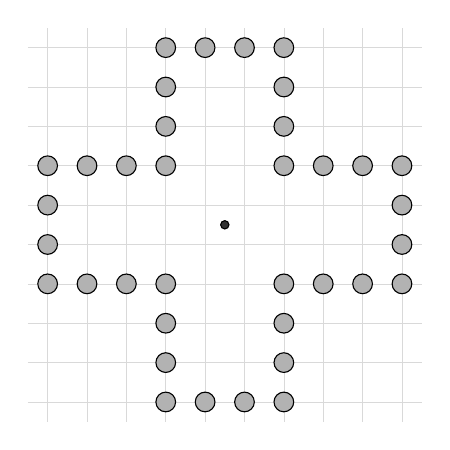
\begin{tikzpicture}
    \drawgrid{-3}{-3}{6}{6}
    \drawmove{-3}{0}{1}{0}
    \drawmove{2}{3}{1}{0}
    \drawcross{0}{0}
    \dotpoint{1.5}{1.5}
    \dotdir{1}{0}{0}
    \dotdir{2}{3}{0}
  \end{tikzpicture}
\end{center}
\end{frame}

\begin{frame}
\frametitle{Additional constraints: move ordering}
Marked Morpion 5D graph $\not\Rightarrow$ Morpion 5D position
\begin{center}
\begin{tikzpicture}
  \CatchFileDef\markedmoves{data/85.moves}{}
  \drawgrid{-4}{-4}{10}{9}
  \foreach \x/\y/\dx/\dy in \markedmoves {
    \drawmove{\x}{\y}{\dx}{\dy}
  }
  \drawcross{0}{0}
  \CatchFileDef\markeddots{data/85.dots}{}
  \foreach \i/\d/\x/\y in \markeddots {
    \dotdir{\x}{\y}{\d}
  }
\end{tikzpicture}
\end{center}
\end{frame}


\begin{frame}
\frametitle{Additional constraints: move ordering}
Additional variable:
\begin{enumerate}
  \setcounter{enumi}{2}
  \item $\ord_v$, $v\in\Bbox$, continuous.\\
  Desired property: $\ord_v\ge\ord_w+1$ if a move $m$ put dot $v$ and
  $w\in m\setminus\{v\}$.
\end{enumerate}

\begin{center}
\begin{tikzpicture}
  \drawgrid{0}{0}{4}{0}
  \drawmove{0}{0}{1}{0}
  \foreach \x in {0, ..., 4} {
    \dotnode{d\x}{\x}{0};
    \ifnum \x = 3
      \dotdir[dot]{\x}{0}{0};
    \else
      \dotmove{\x}{0}
    \fi
  }
  \node[above] at (d1.north) {$w$};
  \node[above] at (d3.north) {$v$};
  \draw[decorate,decoration={brace,amplitude=6pt,mirror,raise=4pt},yshift=-3pt] ([xshift=-5pt]$(d0)$) -- ([xshift=5pt]$(d4)$) node[midway,below,yshift=-9pt] {$m$};
\end{tikzpicture}
\end{center}

Constraint enforcing order on moves:
\begin{block}{}
  \vspace{-15pt}
  \begin{equation}\label{eq:L7}
    \ord_v\ge\ord_w+1-121(1-\mv_{m,v})\quad\text{for each }w\in m\setminus\{v\}\tag*{\L7}
  \end{equation}
\end{block}
\end{frame}

\begin{frame}
\frametitle{Objective}
Maximize the number of moves:
\begin{block}{}
  \vspace{-6pt}
  \begin{equation}\label{eq:Obj}
    \text{maximize}\quad\sum_m\sum_{v\in m}\mv_{m,v}\tag*{{\sffamily Obj}}
  \end{equation}
\end{block}
\end{frame}

\section{Resizing}

\begin{frame}
\frametitle{Feasible and infeasible boxes}
\begin{block}{Feasible box}
  Box $\Bbox$ is \emph{feasible} if mixed integer linear program with conditions \L1--\L5 is feasible,
  i.e. there exists marked Morpion 5D graph fitting box $\Bbox$.
\end{block}
\begin{block}{Infeasible box}
  Box $\Bbox$ is \emph{infeasible} if it is not feasible.
\end{block}
\end{frame}

\begin{frame}
\frametitle{Resized box}
\begin{columns}
\column{.65\textwidth} 
  \begin{center}
  \begin{tikzpicture}
    \drawgrid{-4}{-4}{10}{9}
    \drawcross{0}{0}
    \dotnode{A}{-4}{-4}
    \dotnode{C}{9}{8}
    \draw[dashed,blue] (A) rectangle (C);
    \dotnode{L1}{-4}{1.5}
    \dotnode{L2}{-3}{1.5}
    \draw[<->] (L1.center)--(L2.center) node[midway,above] {1};
    \dotnode{R1}{6}{1.5}
    \alt<1>{\dotnode{R2}{9}{1.5}}{\dotnode{R2}{10}{1.5}}
    \alt<1>{\def\rdist{3}}{\def\rdist{4}}
    \draw[<->] (R1.center)--(R2.center) node[midway,above] {\rdist};
    \dotnode{B1}{1.5}{-4}
    \dotnode{B2}{1.5}{-3}
    \draw[<->] (B1.center)--(B2.center) node[midway,right,yshift=-2pt] {1};
    \dotnode{T1}{1.5}{6}
    \alt<-2>{\dotnode{T2}{1.5}{8}}{\dotnode{T2}{1.5}{9}}
    \alt<-2>{\def\tdist{2}}{\def\tdist{3}}
    \draw[<->] (T1.center)--(T2.center) node[midway,right] {\tdist};
    \only<2>{
      \dotnode{C1}{10}{8}
      \draw[dashed,red] (A) rectangle (C1);
    }
    \only<3>{
      \dotnode{C2}{10}{9}
      \draw[dashed,red] (A) rectangle (C2);
    }
  \end{tikzpicture}
  \end{center}
\column{.35\textwidth}
  \begin{block}{Box by distances}
    We describe a box by a 4-tuple of distances from $\Cross$:
    $(3,2,1,1)$.
  \end{block}
  \begin{block}<2->{Resized box}
    Box {\color{red}$\Bbox$} is \emph{resized} from box {\color{blue}$\Bbox'$}
    if one side is extended by 1 \onslide<1,3>{or two neighboring sides are extended by 1.}
  \end{block}
\end{columns}
\end{frame}

\begin{frame}
\frametitle{Resizing process}
\begin{columns}
\column{.37\textwidth}
\begin{block}{Observation}
  Let $\Bbox$ be a box of a Morpion 5D position.
  There exists $\Bbox'$ s.t. $\Bbox$ is resized from $\Bbox'$
  and there exists Morpion 5D position fitting box $\Bbox'$.
\end{block}
\begin{block}<7>{Corollary}
  If $\Bbox$ is a box of a Morpion 5D position,
  there exists a sequence of feasible boxes $(0,0,0,0)=\Bbox_0,\ldots,\Bbox_n=\Bbox$,
  s.t. $\Bbox_{k+1}$ is resized from $\Bbox_k$.
\end{block}
\column{.63\textwidth}
  \begin{center}
  \begin{tikzpicture}
    \drawgrid{-5}{-4}{9}{10}
    \dotnode{A}{-5}{-4}
    \dotnode<1>{C}{9}{10}
    \dotnode<2>{C}{8}{10}
    \dotnode<3-5>{C}{8}{9}
    \dotnode<6->{C}{8}{8}
    \only<1>{\def\prefix{82}}
    \only<2>{\def\prefix{82_81}}
    \only<3>{\def\prefix{82_80}}
    \only<4>{\def\prefix{82_79}}
    \only<5>{\def\prefix{82_69}}
    \only<6->{\def\prefix{82_68}}
    \draw[dashed,blue] (A) rectangle (C);
    \CatchFileDef\rosindmoves{data/\prefix.moves}{}
    \foreach \x/\y/\dx/\dy in \rosindmoves {
      \drawmove{\x}{\y}{\dx}{\dy}
    }
    \drawcross{0}{0}
    \CatchFileDef\rosinddots{data/\prefix.dots}{}
    \foreach \i/\d/\x/\y in \rosinddots {
      \dotmove{\x}{\y}{\i}
    }
  \end{tikzpicture}
  \end{center}
\end{columns}
\end{frame}

\begin{frame}
\frametitle{The algorithm for resizing process}
\begin{algorithmic}
  \State $\var{unsolved}\gets\{(0,0,0,0)\}$
  \State $\var{solved}\gets\emptyset$
  \While{$\var{unsolved}\neq\emptyset$}
    \State $\Bbox\gets$ pop box from $\var{unsolved}$
    \State $\var{solved}\gets\var{solved}\cup\{\Bbox\}$
    \If{\Call{Solve}{$\Bbox$} is feasible}\Comment{Applying linear solver}
      \ForEach{$\Bbox_{\mathrm{cand}}$ resized from $\Bbox$}
        \Comment{Up to 8 candidates}
        \If{$\Bbox_{\mathrm{cand}}\notin\var{solved}\cup\var{unsolved}$ with respect to symmetries}
          \State $\var{unsolved}\gets\var{unsolved}\cup\{\Bbox_{\mathrm{cand}}\}$
        \EndIf
      \EndFor
    \EndIf
  \EndWhile
\end{algorithmic}
\end{frame}

\section{Results}

\begin{frame}
\frametitle{The hardest feasible boxes}
\begin{center}
%
    \begin{tabular}{|l|l|l|l|}
    \hline
    No &  Bounding box &  Max size  \\
    \hline%
    
1&(3, 4, 1, 1)& 85.0\\
2&(3, 4, 2, 1)& 85.0\\
3&(4, 3, 1, 2)& 85.0\\
4&(4, 3, 1, 3)& 85.0\\
5&(2, 4, 2, 1)& 84.0\\
6&(2, 4, 2, 2)& 84.0\\
7&(2, 5, 1, 2)& 84.0\\
8&(2, 5, 2, 1)& 84.0\\
9&(2, 5, 2, 2)& 84.0\\
10&(3, 3, 1, 2)& 84.0\\
11&(3, 3, 2, 2)& 84.0\\
12&(3, 4, 1, 2)& 84.0\\
13&(3, 4, 1, 3)& 84.0\\
14&(3, 4, 2, 2)& 84.0\\
15&(3, 4, 3, 2)& 84.0\\
16&(4, 3, 0, 2)& 84.0\\
%
    \hline
    \end{tabular}%
\hspace*{5mm}
%
    \begin{tabular}{|l|l|l|l|}
    \hline
    No &  Bounding box &  Max size  \\
    \hline%
    
17&(4, 3, 2, 3)& 84.0\\
18&(2, 3, 2, 1)& 83.0\\
19&(2, 3, 2, 2)& 83.0\\
20&(2, 5, 1, 1)& 83.0\\
21&(3, 2, 1, 2)& 83.0\\
22&(3, 3, 1, 3)& 83.0\\
23&(3, 3, 3, 3)& 83.0\\
24&(3, 4, 2, 3)& 83.0\\
25&(3, 5, 1, 1)& 83.0\\
26&(3, 5, 2, 1)& 83.0\\
27&(4, 3, 0, 3)& 83.0\\
28&(4, 4, 0, 1)& 83.0\\
29&(4, 4, 0, 2)& 83.0\\
30&(4, 4, 1, 1)& 83.0\\
31&(4, 4, 1, 2)& 83.0\\
32&(4, 4, 1, 3)& 83.0\\
33&(4, 5, 1, 2)& 83.0\\
%
    \hline
    \end{tabular}%

\end{center}
\end{frame}

\begin{frame}
\frametitle{Upper bound of 84}
For three bounding boxes with $\textrm{Size}=85.0$
we run solver again with added constraint \L7.\\
It was able to reduce upper bound below 85.
\vspace{2cm}

\pause
Using the same process we prove that the best score for symmetric Morpion 5D is 68
(found by M.~Quist in 2008).\\

\end{frame}

\appendix

\backupbegin

\section{\appendixname}

\begin{frame}
\frametitle{Progress in proving upper bound of 82}
\url{https://github.com/anagorko/morpion-lpp/wiki/Solving-5D}
\end{frame}

\backupend

\end{document}
